%!TEX root = ../../thesis_master.tex

%%%%%%%%%%
\chapter{Implementation}
\label{chap:implementation}
%%%%%%%%%%

In this chapter, the implementation details of the system previously described are given.

All the elements of the system have been implemented as ROS components using its C++ API. The code is organized as a stack called \texttt{flypulator\_vs} and composed of five ROS packages described below. All the source code is available on GitHub\footnote{\url{https://github.com/PabloRdrRbl/flypulator_vs}} under a GPLv3 license\footnote{\url{https://github.com/PabloRdrRbl/flypulator_vs/blob/master/LICENSE}}. The content of each of the following ROS packages is the following:

\nomenclature[ba]{API}{Application Programming Interface}

\begin{itemize}
	\item \texttt{flypulator\_vs\_controller}: Contains the action server for the visual servo controller. The node receives a desired marker and pose, conducts the corresponding visual servoing task and publishes the velocities to the robot command topic. Additionally the action server publishes feedback about the current task.
	
	\item \texttt{flypulator\_vs\_demo}: Contains the ROS launch files to run all the components needed for a demonstration of the controller.
	
	\item \texttt{flypulator\_vs\_gazebo}: Contains the URDF files for the markers and the world used during the simulation.
	
	\item \texttt{flypulator\_vs\_msgs}: Contains the descriptor of the action interface.
	
	\item \texttt{flypulator\_vs\_task}: Contains the action client for the visual servo controller. The node is used to get the user input for the selection of the desired marker and pose. The desired pose is specified in a text file, while the desired marker is selected by the user by clicking on one of the currently available makers in the camera image. The user input is published so the action server can receive it.
\end{itemize}

All the C++ code follows the ROS Style Guide \cite{ROS_Style} and has been conveniently documented using the Doxygen\footnote{\url{http://www.stack.nl/~dimitri/doxygen/}} documentation generator tool.

In the following sections, the most relevant aspects of the implementation are discussed. These are: 

\begin{itemize}
	\item How are the hardware and environment simulated?
	
	\item How is the target detection and tracking conducted?
	
	\item How is the visual servoing algorithm implemented?
	
	\item How is the system integrated as a ROS component?
\end{itemize}


\section{Gazebo Simulation}
\label{sec:gazebo-simulation}

It has been already explained how ROS works as an operating system for the robot, allowing the complete implementation of a robotic system. This is valid not only for real hardware, but also for simulated robots. In order to do that, an additional tool is needed to work along with ROS. This is the roll of the Gazebo robotics simulator.

Gazebo is a 3D dynamic simulator used to simulate robotic environments. It allows the kinematic and dynamic simulation of robots and other bodies, indoor and outdoor environments with different illumination conditions and textures and the emulation of sensors such as cameras or light rangers. Additionally, using the Gazebo plug-in's it is possible to model more complex phenomenas including, aerodynamics or controllers.

\emph{Gazebo} works as an additional ROS node. It subscribes to the topics containing the robot's current state and publishes in other topics the new state of the robot. An example of this architecture is shown in Figure \ref{fig:gazebo_example}.

\begin{figure}[!htb]
	\caption{Example of a simple communication between Gazebo and the rest the ROS environment of a quadrotor simulation}
	\centering
	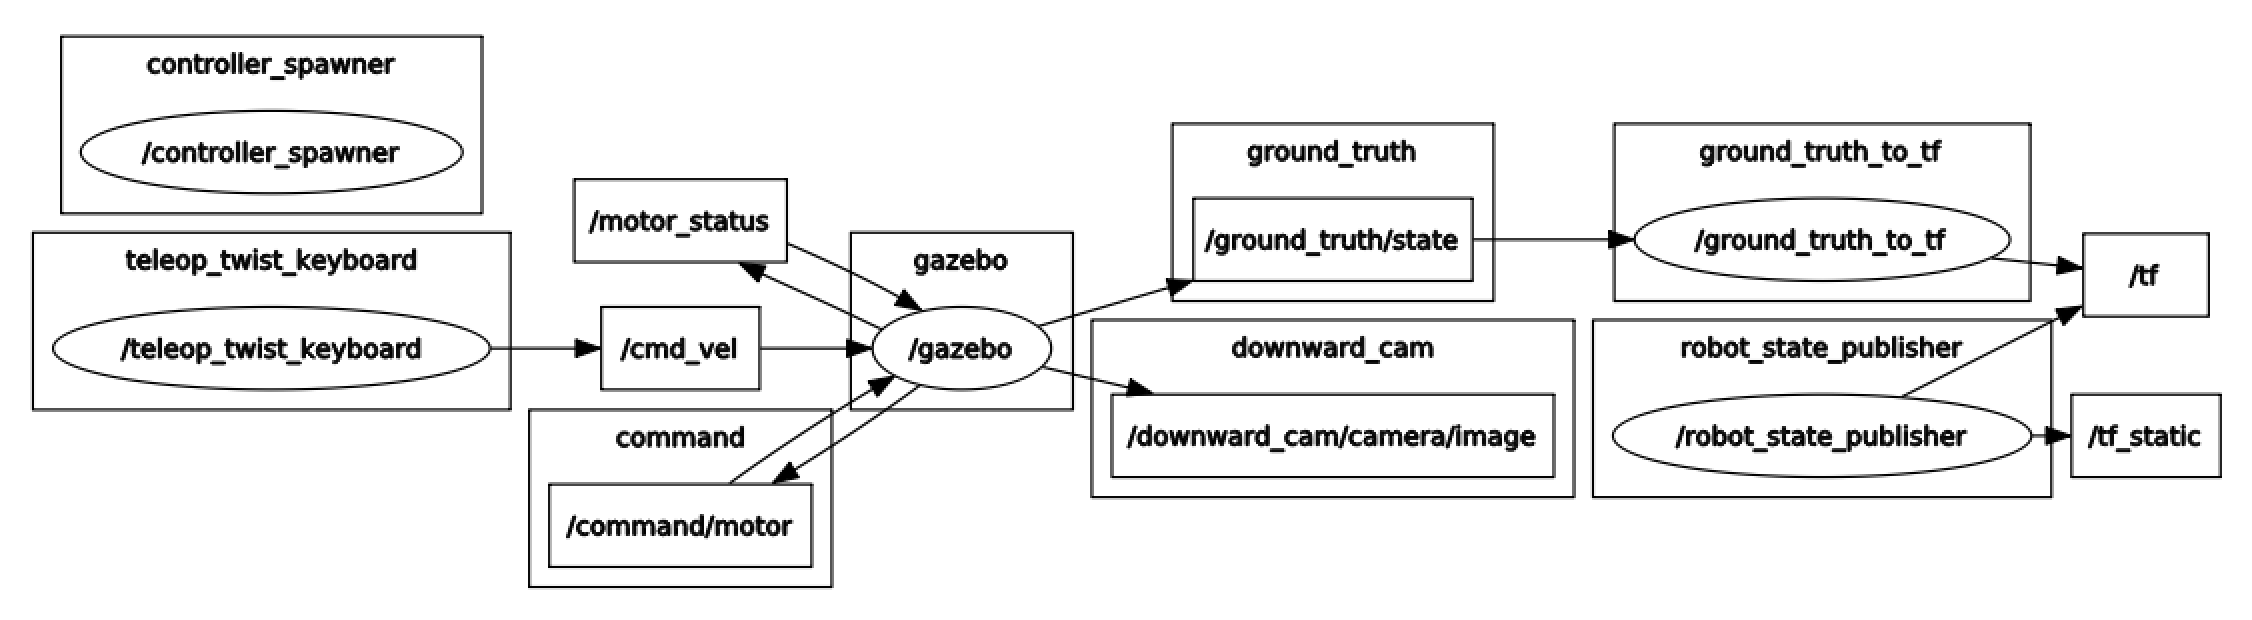
\includegraphics[width=\textwidth]{content/chapter_05/images/gazebo_example.png}
	\label{fig:gazebo_example}
\end{figure}

In order to use a robot in \emph{Gazebo}, it is necessary to convert its CAD files to the \emph{Unified Robot Description Format} (URDF). This is an XML format for representing a robot model. A similar procedure is also followed to introduce any other model in the simulation, for example the target markers.

\nomenclature[ba]{CAD}{Computer Aided Design}
\nomenclature[ba]{URDF}{Unified Robot Description Format}

Once the robot and the markers have been spawned in the desired world (Gazebo's scenes) the simulator publishes data such as the camera images or the robot state and subscribes to the velocity commands and motor status of the robot. In this manner, it is possible to simulate not only the robot dynamics due to the input commands, but also the sensor data readings of the robot for this state (e.g. the camera image).

For this work, the quadrotor \texttt{hector\_quadrotor}\footnote{\url{http://wiki.ros.org/hector_quadrotor}} has been used. It contains not only the robot description in form of URDF files, but also the low-level controllers necessary to command the robot via kinematic inputs. The desired linear and angular velocities are published to the \texttt{\textbackslash cmd\_vel} topic the low-level controllers, which compute the necessary motor inputs and allow the control ot the translation and yaw of the robot. Additional, the quadrotor has an on-board camera pointing downwards, which is simulated by Gazebo, who publishes into two topics\footnote{In the code the topics are called respectively \texttt{\textbackslash camera\textbackslash image} and \texttt{\textbackslash camera\textbackslash info} for compatibility with other robots. The mentioned names are remapped where the visual servo controller is launched.}:

\begin{itemize}
	\item \texttt{\textbackslash downward\_camera\textbackslash camera\textbackslash image}: Contains the camera image simulated by Gazebo.
	
	\item \texttt{\textbackslash downward\_camera\textbackslash camera\textbackslash info}: Contains the camera intrinsic parameters.
\end{itemize}

The \texttt{flypulator\_vs\_gazebo} package contains all launch files to start the Gazebo simulation under the directory \texttt{\textbackslash launch}. The \texttt{hector\_quadrotor} stack is installed separately and called by the launch file \texttt{start.launch}. Any other robot could be spawned in a similar manner.

\section{ViSP Visual Servoing Framework}
\label{sec:visp}

ViSP\footnote{\url{https://visp.inria.fr}} (\emph{Visual Servoing Platform}) is a visual servoing open source framework for the development of visual tracking and visual servoing systems created by the Inria Lagadic\footnote{\url{http://team.inria.fr/lagadic/}} team. ViSP allows the computation and tracking of visual features, the design of control laws for a robotic system and other computer vision tools \cite{visp_hp}.

\nomenclature[ba]{ViSP}{Visual Servo Platform}

The library is written in C++ and distributed for different platforms. It is provides a \texttt{vpServo} class which contains all the elements of a classical visual servoing control algorithm. The Listing \ref{simple-visp} contains a code snippet with a simple visual servoing task using ViSP.

The framework contains a class for each of the common visual features, including the computation of their interaction matrix as explained in Section \ref{sec:image-moments}. ViSP is thoroughly documented, so the reader is recommended to consult the online documentation\cite{visp_doc} for further details. In the case of this work, the features used are implemented in the classes \texttt{vpFeatureMomentAreaNormalized} and \texttt{vpFeatureMomentGravityCenterNormalized }.

The communication between the library and ROS is established via the \texttt{visp\_ros}\footnote{\url{http://wiki.ros.org/visp_ros}} package. The class \texttt{vpROSGrabber} subscribes to the camera image and camera info topics and converts the image from the camera into a format compatible with ViSP. While the class \texttt{vpROSRobot} allows publishing directly to the velocity command topic. It allows ViSP to be run outside the ROS node if desired, although this would result in less integration of the algorithm. The implementation proposed integrates ViSP inside a ROS node, as described in Figure \ref{fig:visual-servo-ros-node}.
  
\ifalisting{Simple ViSP example}{simple-visp}{c++}{none}{content/chapter_05/listings/visp_simple_example.cpp}{true}

\begin{figure}[!htb]
	\caption[Architecture of ViSP running inside a ROS node]{Architecture of ViSP running inside a ROS node~\protect\cite{visp_ros}}
	\centering
	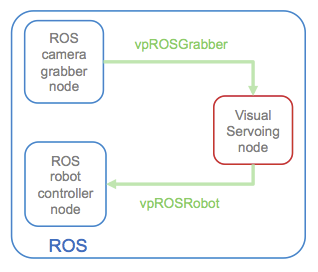
\includegraphics[width=0.4\textwidth]{content/chapter_05/images/visual-servo-ros-node.png}
	\label{fig:visual-servo-ros-node}
\end{figure}

\section{AprilTag Markers}
\label{sec:apriltag_markers}

AprilTag\footnote{\url{https://april.eecs.umich.edu/software/apriltag/}} is a visual fiducial system, useful for a wide variety of tasks including augmented reality, robotics and camera calibration. Targets can be created from an ordinary printer, and the AprilTag detection software computes the precise 3D position, orientation, and identity of the tags relative to the camera \cite{apriltag_hp}. 

In this work, AprilTag markers have been used as target. Any detected AprilTag can be used to compute the relative pose between the camera and the marker frame of reference. Since the IBVS algorithm does not use any pose computation, here only the marker detection is used. Once the marker has been detected, the detector returns a list of the camera coordinates of the corners of the marker ordered clock-wise and starting in the bottom-left cornet of the tag, as indicated in Figure \ref{fig:april-frames}.

\begin{figure}[!htb]
	\caption{Example of simple communication between Gazebo and ROS}
	\centering
	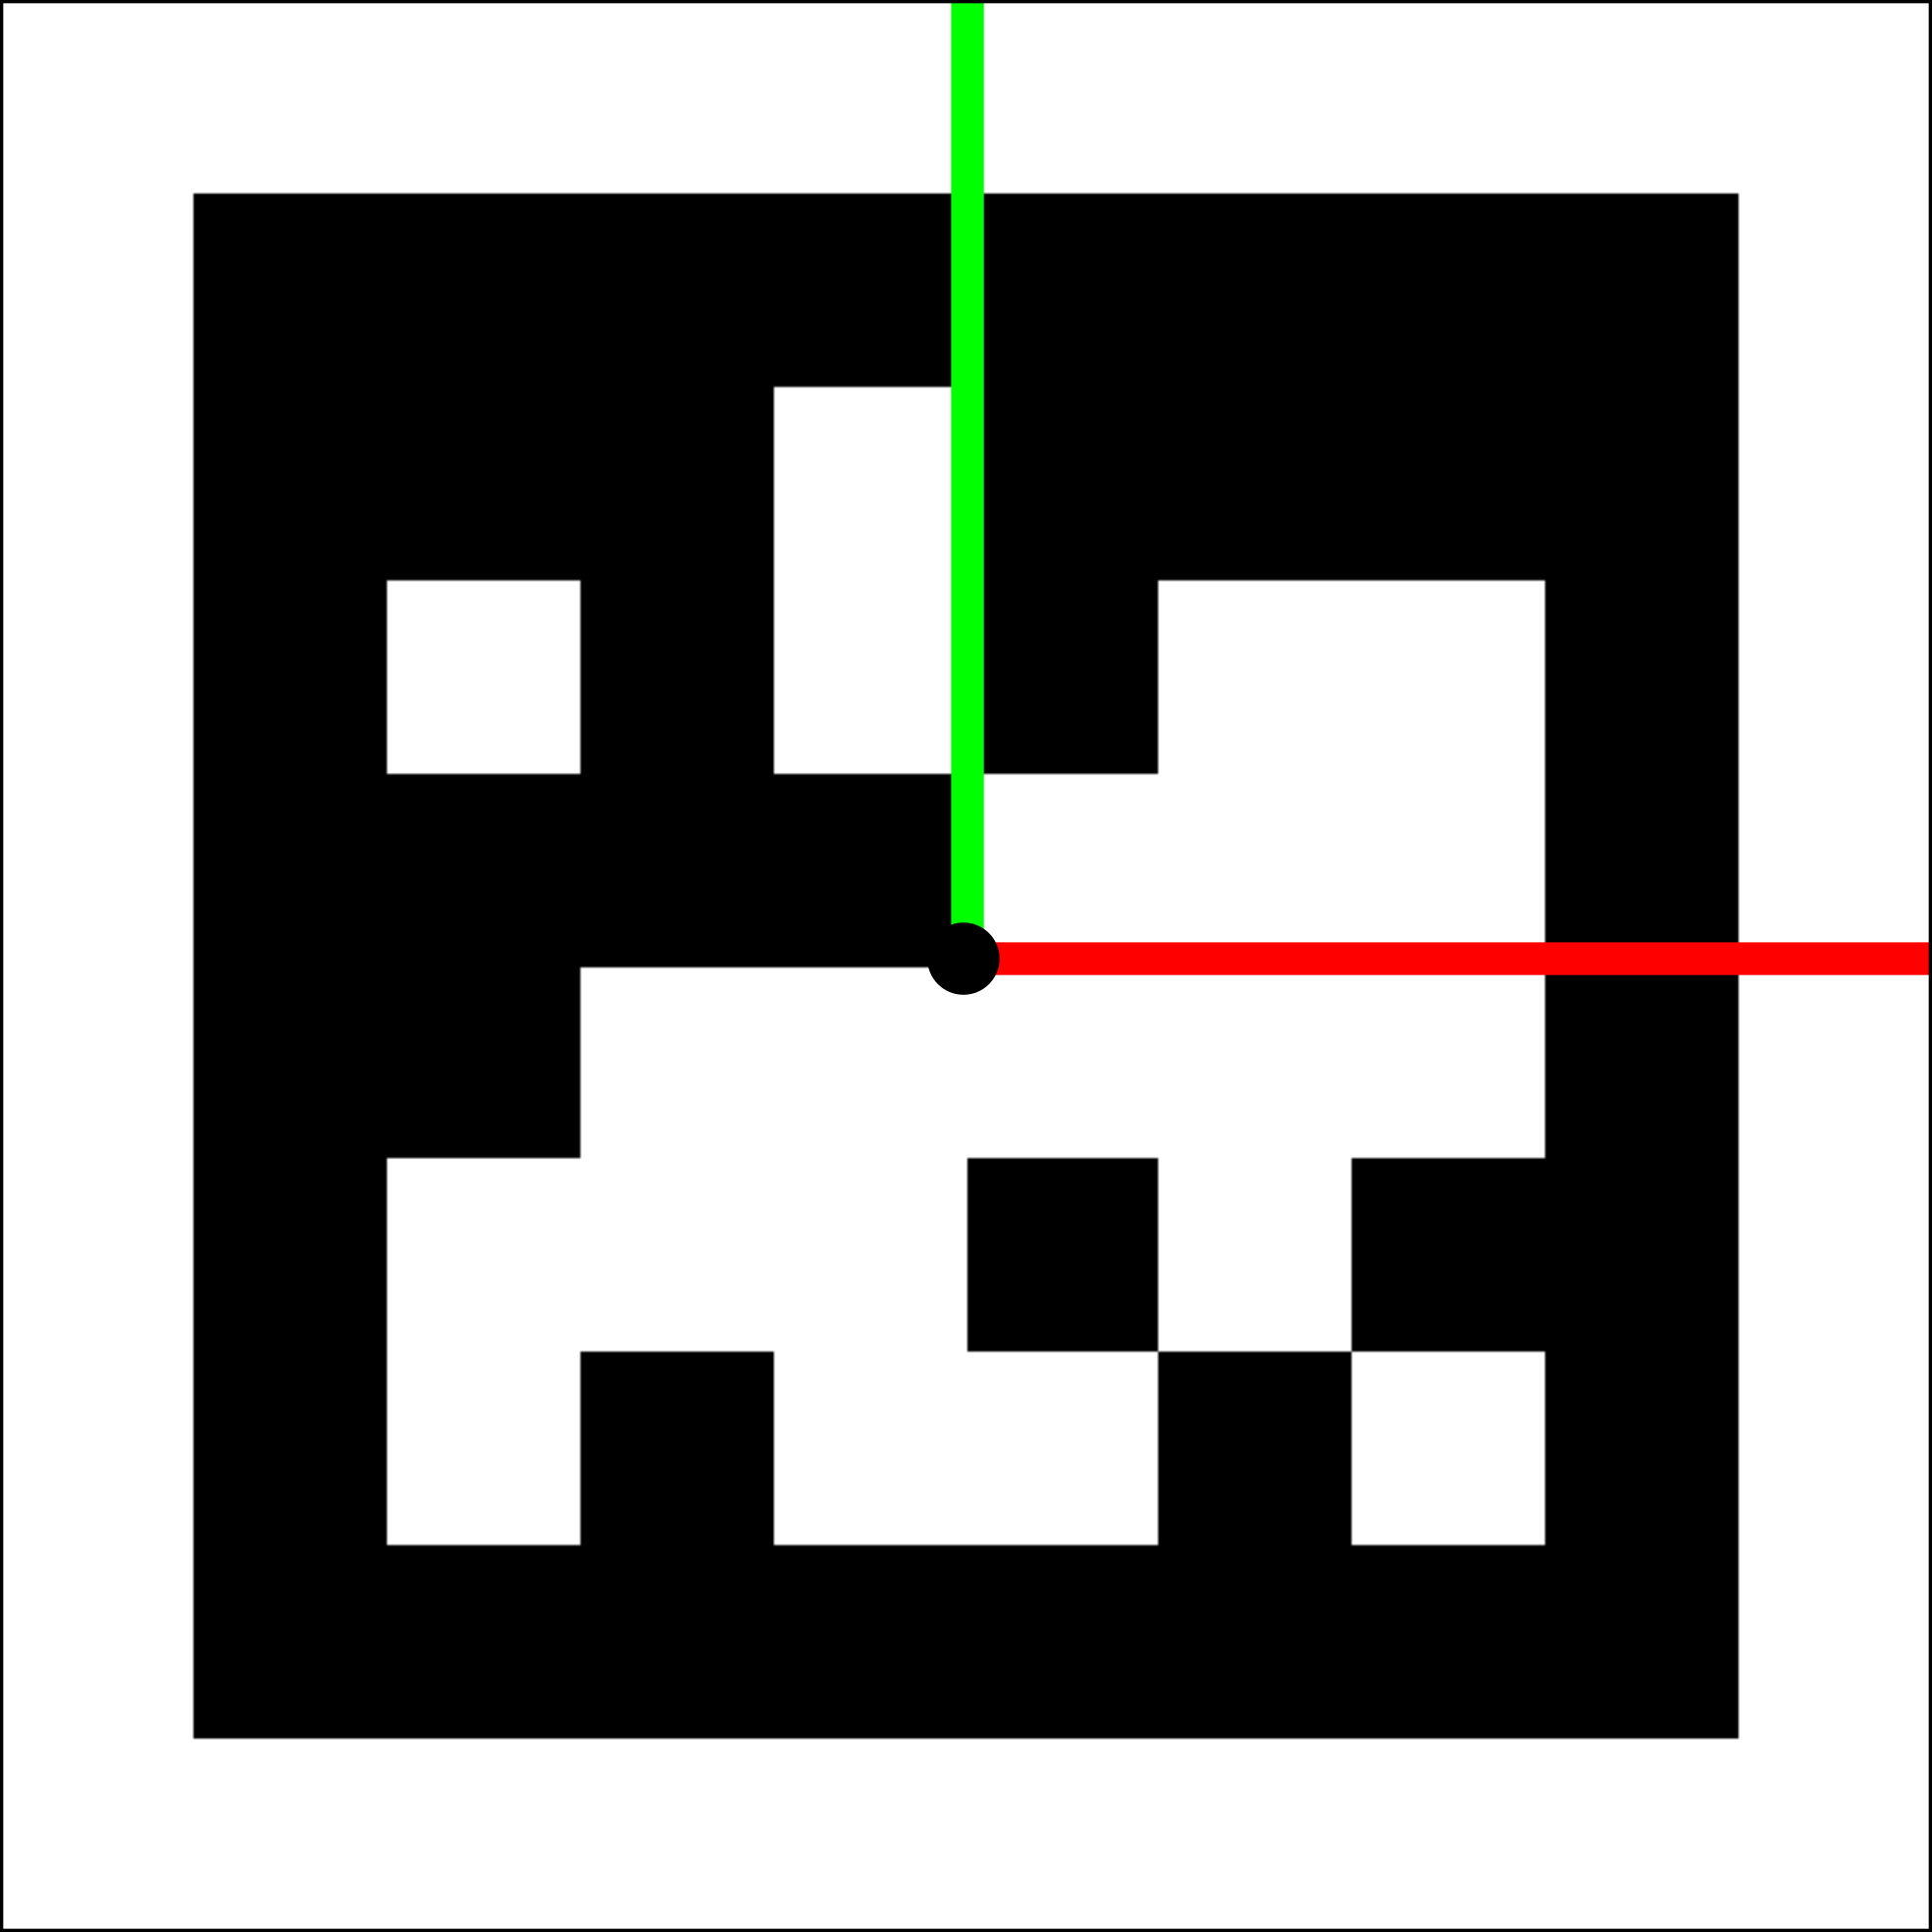
\includegraphics[width=0.4\textwidth]{content/chapter_05/images/april-frames}
	\label{fig:april-frames}
\end{figure}

The AprilTag detector is provided by the creators of the tags and implemented  in different programming languages. Here the \texttt{vpDetectorAprilTag} detector wrapper provided in ViSP is used. 

\ifalisting{Simple AprilTag detection example}{example-april}{c++}{none}{content/chapter_05/listings/apriltag_detector_example.cpp}{true}

Once the four corners of the marker are detected, it is possible to compute the image features as described in Chapter \ref{chap:system-design}. The marker tracking is not necessary, since it is not moving it is just detected every cycle of the control algorithm. The markers are arranged in families (the implementation uses the \texttt{36h11} family), so different makers can be present in the camera image. The detector detects all of them, so the user can access each of them using their respective ID. Figure \ref{fig:apriltag-detection} shows the detection of two different target during a simulation, as well as the tagets' IDs.

\begin{figure}[!htb]
	\caption{AprilTag detection in a multi-target image}
	\centering
	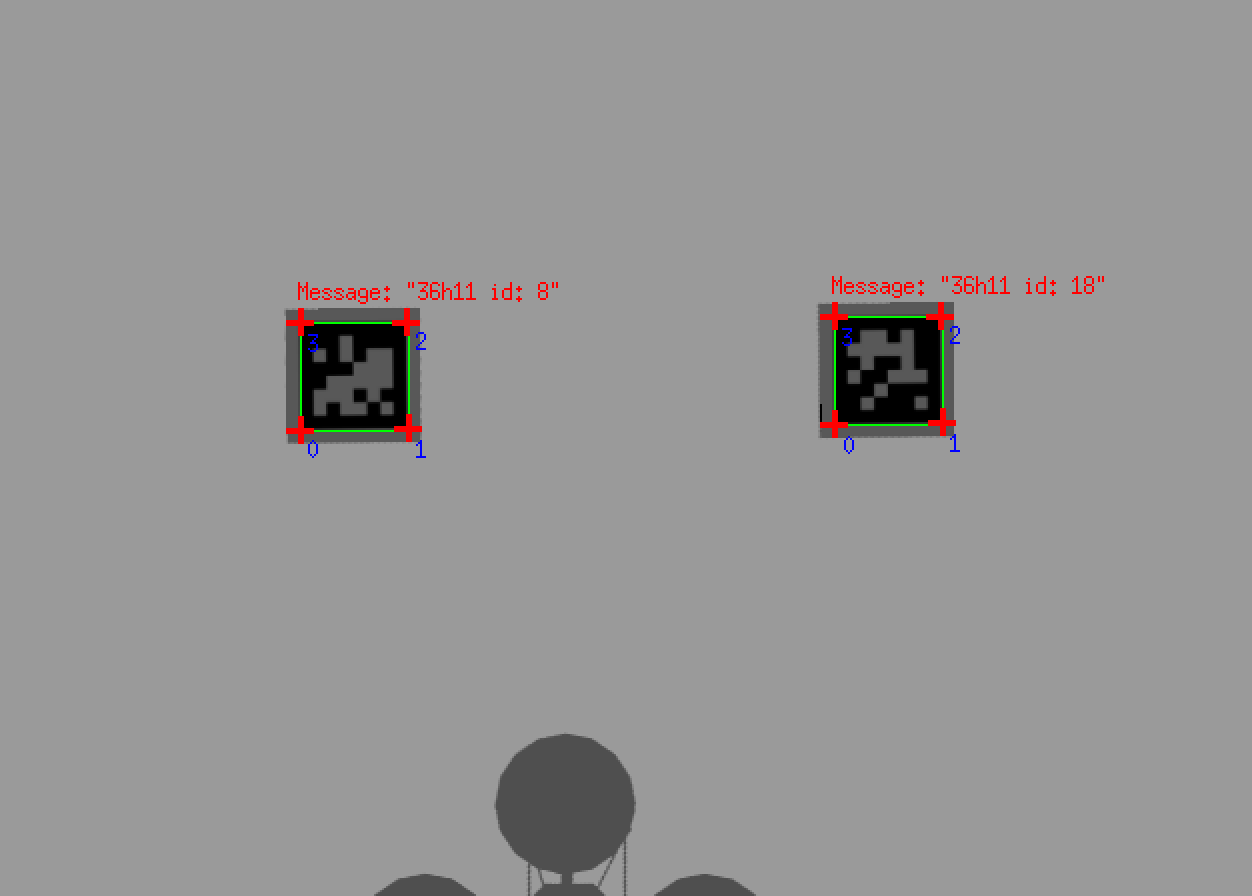
\includegraphics[width=0.7\textwidth]{content/chapter_05/images/april-detection.png}
	\label{fig:apriltag-detection}
\end{figure}

The possibility of having several markers is very useful for manipulation tasks, where several objects can be together. In this case, the system could select a target among all the present possibilities. In order to select a target, the system only needs the ID of the desired marker. This can be obtained from a user click, a data base relating IDs and objects or a text file.

 In order to integrate the AprilTag's markers in Gazebo, a cube of dimensions $25\text{cm}\times25\text{cm}\times1\text{mm}$ was created in Blender\footnote{\url{https://www.blender.org}}. For each marker, the AprilTag image was rescaled to the dimension of the cube's face and applied as texture of the cube using the \emph{UV Unwrapping} tool. The Blender object was finally exported as a COLLADA file. All the Gazebo implementation of the AprilTags is in the \texttt{flypulator\_vs\_gazebo} package. The COLLADA file is spawned as URDF file using the \texttt{generic\_spawn.launch} launch file.

\begin{figure}[!htb]
	\caption{Quadrotor flying over two AprilTags in a Gazebo simulation}
	\centering
	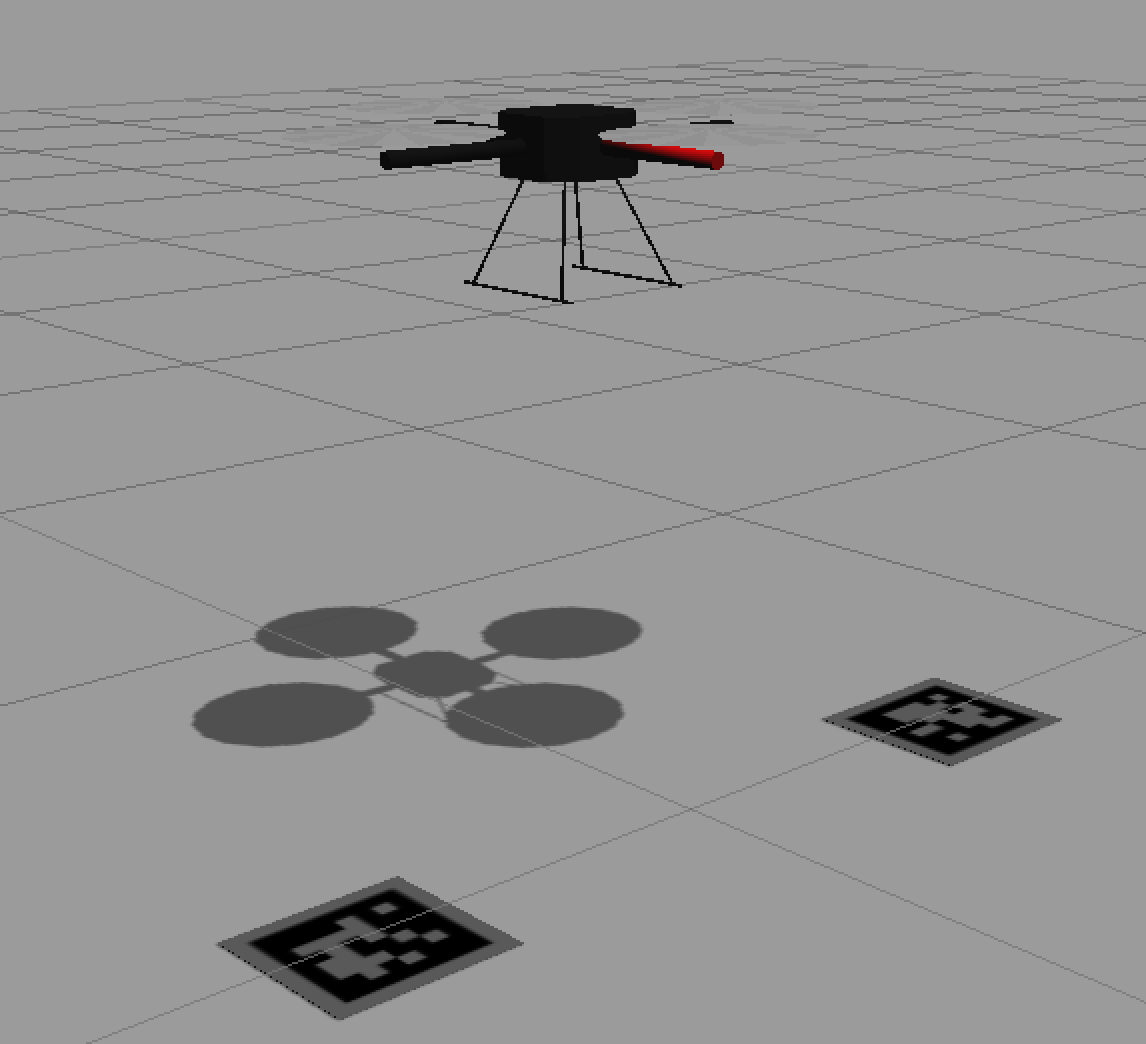
\includegraphics[width=0.5\textwidth]{content/chapter_05/images/fly2tags.png}
	\label{fig:fly2tags}
\end{figure}

\section{ROS Action Interface}
\label{sec:ros_action}

In this section, the action interface created for the visual servo controller is described. The purpose of this interface is to separate the task creation by the user and the task execution in the controller. The action interface is provided by ROS in the \texttt{actionlib}\footnote{\url{http://wiki.ros.org/actionlib}} package.

The action interface comprises two agents, the action client and the action server. The action server is always running, waiting for the client to send a new task (a new \emph{action}).

An action \cite{ROS_ComPat} is an abstraction of a discrete behavior that moves the robot or runs for a longer time, producing feedback during the execution. Examples of possible actions are moving the arm of a robot to a certain pose, pointing the head of a robot into a desired point or performing a laser scan. In this case, the action is commanding the aerial robot towards the desired pose with respect to the target using a visual servoing algorithm.

Using an action interface has several advantages with respect to the other communication methods provided in ROS. An alternative implementation could be running the entire visual servo controller in a unique node. The node could be launched using a service and the feedback could be published into a topic. But services block the communication while there are running and shut down when they are finished, they are though to a short task like switching on the robot motors. While the action can be preempted in any moment, e.g. when another goal is sent by a other client, and the server keeps waiting for a new goal. Furthermore, the action interface allows the separation of the goal generation and the goal search. Services can be used to start the low-level controllers of the robot at the start of the simulation, since the low-level controllers are activated only one and keep running all the time. While the action allows the visual servoing task to be started several times during the robot's operation.

 Each action is defined by three elements if form of messages on which the server and client communicate: the \emph{goal}, \emph{feedback} and \emph{result}. These messages are created in de \emph{action descriptor}. The action descriptor for the IBVS action is placed in the package \texttt{flypulator\_vs\_msgs} within the directory \texttt{\textbackslash action} in a file called \texttt{AprilTagIBVS.action} and reproduced in the Listing \ref{AprilTagIBVS}. For each of the three elements, one or more variables are created, each of them defined by a message type and a name.

\ifalisting{Action descriptor for the IBVS task}{AprilTagIBVS}{C++}{none}{content/chapter_05/listings/AprilTagIBVS.action}{true}

The action server is implemented within the \texttt{flypulator\_vs\_controller} as a node called \texttt{vs\_action\_server}. It contains the ViSP code to execute the IBVS task based on the goal provided to it. The code is structured around the class \texttt{VisualServoingServer}. The class constructor receives the parameters of the servo controller from the ROS Parameter Server and subscribes to the robot command and camera topics. Finally it starts the action server.

Every time that the action server receives a new request from the client, the method \texttt{executeCB} is used as callback, running the visual servoing task. During the servo task, the node publishes feedback in the \texttt{\textbackslash vs\_action\textbackslash feedback} topic, where the feedback is in this case the current error of the control law. When the tolerance of the control error has been achieved, the control law stops the robot and terminates and the server publishes the last control error in the \texttt{\textbackslash vs\_action\textbackslash result}. Additionally, the server tells the client that the task was finished. So the client can shut down while the server keeps running waiting for another client request. In Figure \ref{fig:action_interface}, the basic architecture of the action interface is presented, while Figure \ref{fig:action_interface_ros} shows a part of the ROS network while the visual servoing controller is running.

\begin{figure}[!htb]
	\caption{Basic architecture of the implemented action interface}
	\centering
	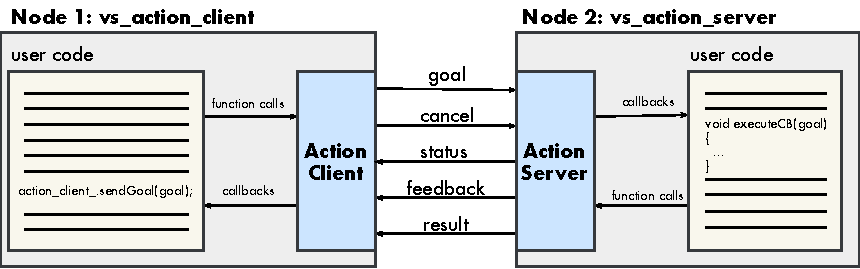
\includegraphics[width=\textwidth]{content/chapter_05/images/action_interface.pdf}
	\label{fig:action_interface}
\end{figure}

In order to set a concrete goal for the action server a client is necessary. The goal assignation is completely independent from the servo control implementation, i.e. the user can write a new client to assign the goal according to his/her respective needs. The only requirement is that the node runs a client using the class \texttt{SimpleActionClient} provided by the \texttt{actionlib} package and the action message type created in the action descriptor. A simple implementation of a client for the IBVS controller is presented in the Listing \ref{simple_action_server}.

However, for this work a more complex client was written. When the client launches the current image seen by the camera is displayed, so the user can click the desired AprilTag. The desired pose is prescribed using the quaternion from the traget's reference system $O$ to the camera optical frame $C$, as in the previous example. This implementation is contained in the package \texttt{flypulator\_vs\_client} within the class \texttt{VisualServoingClient}.

\ifalisting{Simple action server for the IBVS controller}{simple_action_server}{C++}{none}{content/chapter_05/listings/simple_action_client_example.cpp}{true}

\begin{figure}[!htb]
	\caption{Example of ROS network while running the robot simulation and the visual servo controller}
	\centering
	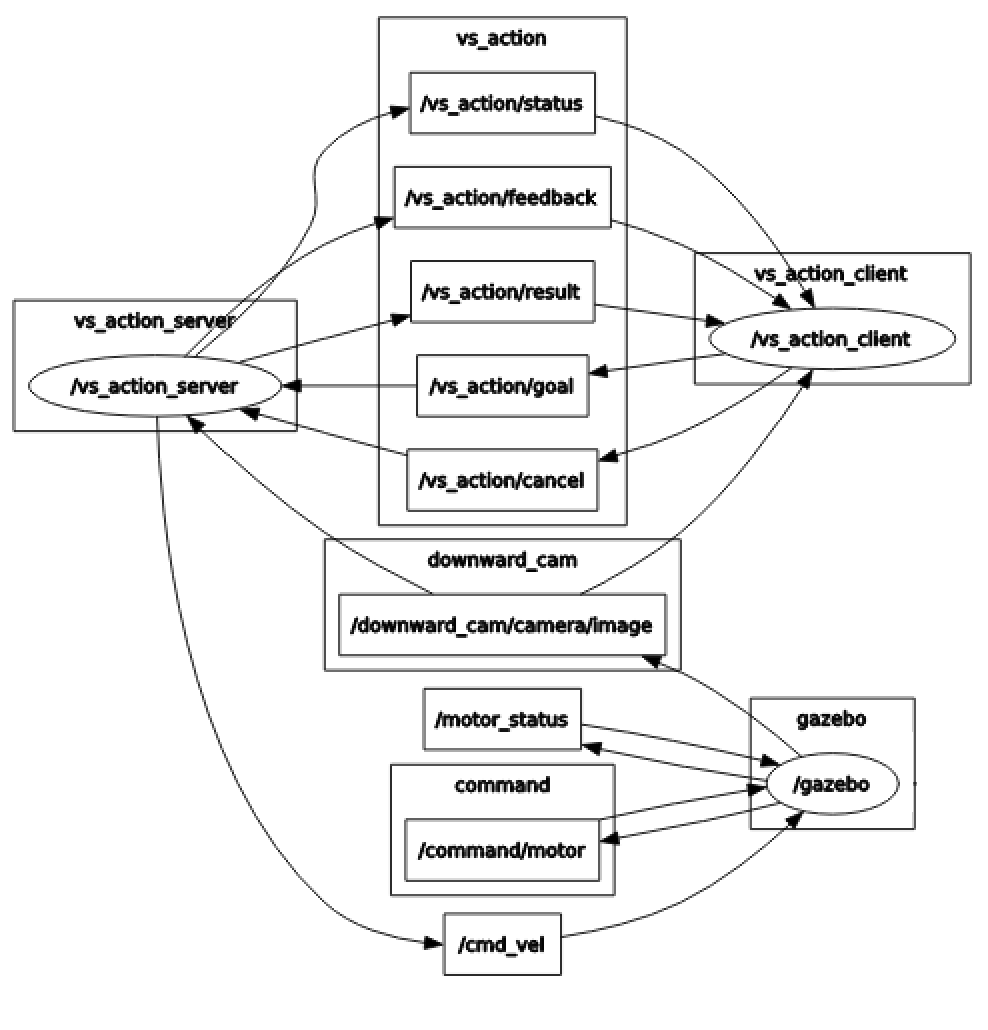
\includegraphics[width=\textwidth]{content/chapter_05/images/action_interface_rqt.png}
	\label{fig:action_interface_ros}
\end{figure}

\section{Controller Parameter Server}
\label{sec:parameter_server}

The ROS Parameter Server\footnote{\url{http://wiki.ros.org/Parameter\%20Server}}  is used to allow to modify the controller's gain. As already explained in Section \ref{sec:ROS_theory}, the Parameter Server allows a the centralized data storage in form of dictionary structure. 

New parameters can be added in form of a YAML\footnote{\url{http://yaml.org}} file. YAML is a human-readable data serialization language commonly used for configuration files. For the visual servo controller this file is located in the package \texttt{flypulator\_vs\_controller} within the directory \texttt{\textbackslash params} in a file called \texttt{params.yaml} and reproduced in the Listing \ref{vs_params}.

\ifalisting{Configuration file for the parameters of the visual servo controller}{vs_params}{}{none}{content/chapter_05/listings/params.yaml}{true}

The parameters are published under a given name space, in this case the \texttt{vs\_parameter\_server\_namespace}. Additional levels can be defined within the YAML file. The desired parameters are written in the file which is loaded in the ROS network through the following line in the launch file (see Listing \ref{vs_launch}).

 To access the data from a given node, the \texttt{ros::NodeHandle::param()} method is used. 

\ifalisting{ROS launch file for the visual servo controller action server}{vs_launch}{XML}{none}{content/chapter_05/listings/vs_controller.launch
}{true}